%!TEX root = ../thesis.tex
%*******************************************************************************
%*********************************** Background estimation *********
%*******************************************************************************


\chapter{Background estimation}\label{ch:background_estimation}

\ifpdf
    \graphicspath{{chapter-background/Figs/Raster/}{chapter-background/Figs/PDF/}{chapter-background/Figs/}}
\else
    \graphicspath{{chapter-background/Figs/Vector/}{chapter-background/Figs/}}
\fi

\glsreset{cr}

A reliable and trustworthy estimation of the expected \gls{sm} background rates in the signal regions is crucial for exercising the statistical machinery laid out in \cref{ch:statistics} and making conclusive statistical statements about the \gls{susy} scenarios studied. The background estimation approaches used herein either rely on semi-data-driven techniques, or on \gls{mc}-only estimations. As estimating backgrounds only from \gls{mc} simulation is sometimes problematic due to \eg mis-modelings in the phase space targeted not being appropriately covered by the uncertainties, a (semi-)data-driven approach is often favoured. In the following, the major backgrounds $\ttbar$, single top and $\wjets$ are estimated using a semi-data-driven approach, while the expected rates from the remaining, smaller backgrounds rely purely on \gls{mc} simulations and are normalised to their theoretical cross section.

\section{General strategy}

\subsection{Transfer factor approach}

Estimating background contributions in \glspl{sr} in a semi-data-driven approach usually involves the introduction of so-called \glspl{cr} ,used to control dominant background processes by comparing their expected event rates to data. The \glspl{cr} are designed to be enriched in events of a given background process (or type) while being approximately free of signal contamination. If $N_p^\mathrm{MC}(\mathrm{SR})$ and $N_p^\mathrm{MC}(\mathrm{CR})$ are the expected rates for a given background process $p$ obtained from \gls{mc} simulation in a given \gls{sr} and \gls{cr}, respectively, then the transfer factor $N_p^\mathrm{MC}(\mathrm{SR})/N_p^\mathrm{MC}(\mathrm{CR})$ allows to convert the number of observed background events in the \glspl{cr}, $N_p^\mathrm{obs.}(\mathrm{CR})$, into a background estimate in the \glspl{sr}, $N_p^\mathrm{est.}(\mathrm{SR})$, through
\begin{equation}
	N_p^\mathrm{est.}(\mathrm{SR}) = N_p^\mathrm{obs.}(\mathrm{CR}) \frac{N_p^\mathrm{MC}(\mathrm{SR})}{N_p^\mathrm{MC}(\mathrm{CR})} = \mu_p N_p^\mathrm{MC}(\mathrm{SR}).
	\label{eq:transfer_factor}
\end{equation}
Here, $\mu_p$ is the process-specific normalisation factor introduced in~\cref{sec:likelihood_function}. An important benefit of this approach is that the impact of systematic uncertainties on the estimated background rates can be evaluated on the transfer factors, that are ratios of \gls{mc} estimates. As such, systematic uncertainties can cancel in the extrapolation to the \glspl{sr}. The uncertainty on the background estimate in the \glspl{sr} is then a combination of statistical uncertainties in the \glspl{cr} and remaining uncertainties affecting the extrapolation~\cite{HistFitter:2014wma}. For this reason, \glspl{cr} are usually deliberately chosen to have large statistics, effectively reducing the uncertainties on the extrapolation to the \glspl{sr}.  

As indicated in~\cref{eq:transfer_factor}, the transfer factor approach is formally equivalent to using the process-specific normalisation factors from~\cref{sec:likelihood_function}, effectively \textit{normalising} the number of total background events expected from \gls{mc} simulation to the number of observed events in each control region. In the profile likelihood fits used in the following, implemented using \textsc{HistFitter}~\cite{HistFitter:2014wma}, the normalisation factors $\mu_p$ are fitted to data instead of the background processes as expected from \gls{mc} simulation. Multiple disjoint \glspl{cr} are used to simultaneously normalise multiple background processes to data in a combined fit. In order not to have an underdetermined minimisation problem, at least the same number of \glspl{cr} as normalisation factors need to be used. Two different profile likelihood fit configurations are used in the following; the first configuration being a so-called \textit{background-only} fit configuration, assuming no signal contribution and typically only including the \glspl{cr}. The second configuration is a so-called \textit{model-dependent} fit configuration with nominal signal contribution using all \glspl{cr} as well as \glspl{sr}.

In order to verify the quality of the extrapolation from the \glspl{cr} to the \glspl{sr}, so-called \glspl{vr} are defined. \glspl{vr} do not participate in the actual fit of the model parameters to data, but serve as intermediate regions to verify the extrapolation. For this reason, \glspl{vr} are typically placed in the region between the \glspl{cr} and \glspl{sr} that is extrapolated over. A schematic view of an analysis strategy using all three types of regions is shown in~\cref{fig:hf_strategy}. All three types of regions can have more than one bin and are separated using suitable observables that are extrapolated over. In order to be able to use information from all control and signal regions in a single profile likelihood fit, all regions necessarily need to be statistically independent.

\begin{figure}
\floatbox[{\capbeside\thisfloatsetup{capbesideposition={right,center},capbesidewidth=0.5\textwidth}}]{figure}[\FBwidth]
{\caption{Schematic view of an analysis strategy including multiple control, validation and signal regions with one or multiple bins each. Extrapolations from the control regions into the signal regions can be verified in the validation regions lying in the phase space extrapolated over. All regions are designed to be statistically independent. Figure adapted from~\cite{HistFitter:2014wma}.}\label{fig:hf_strategy}}
{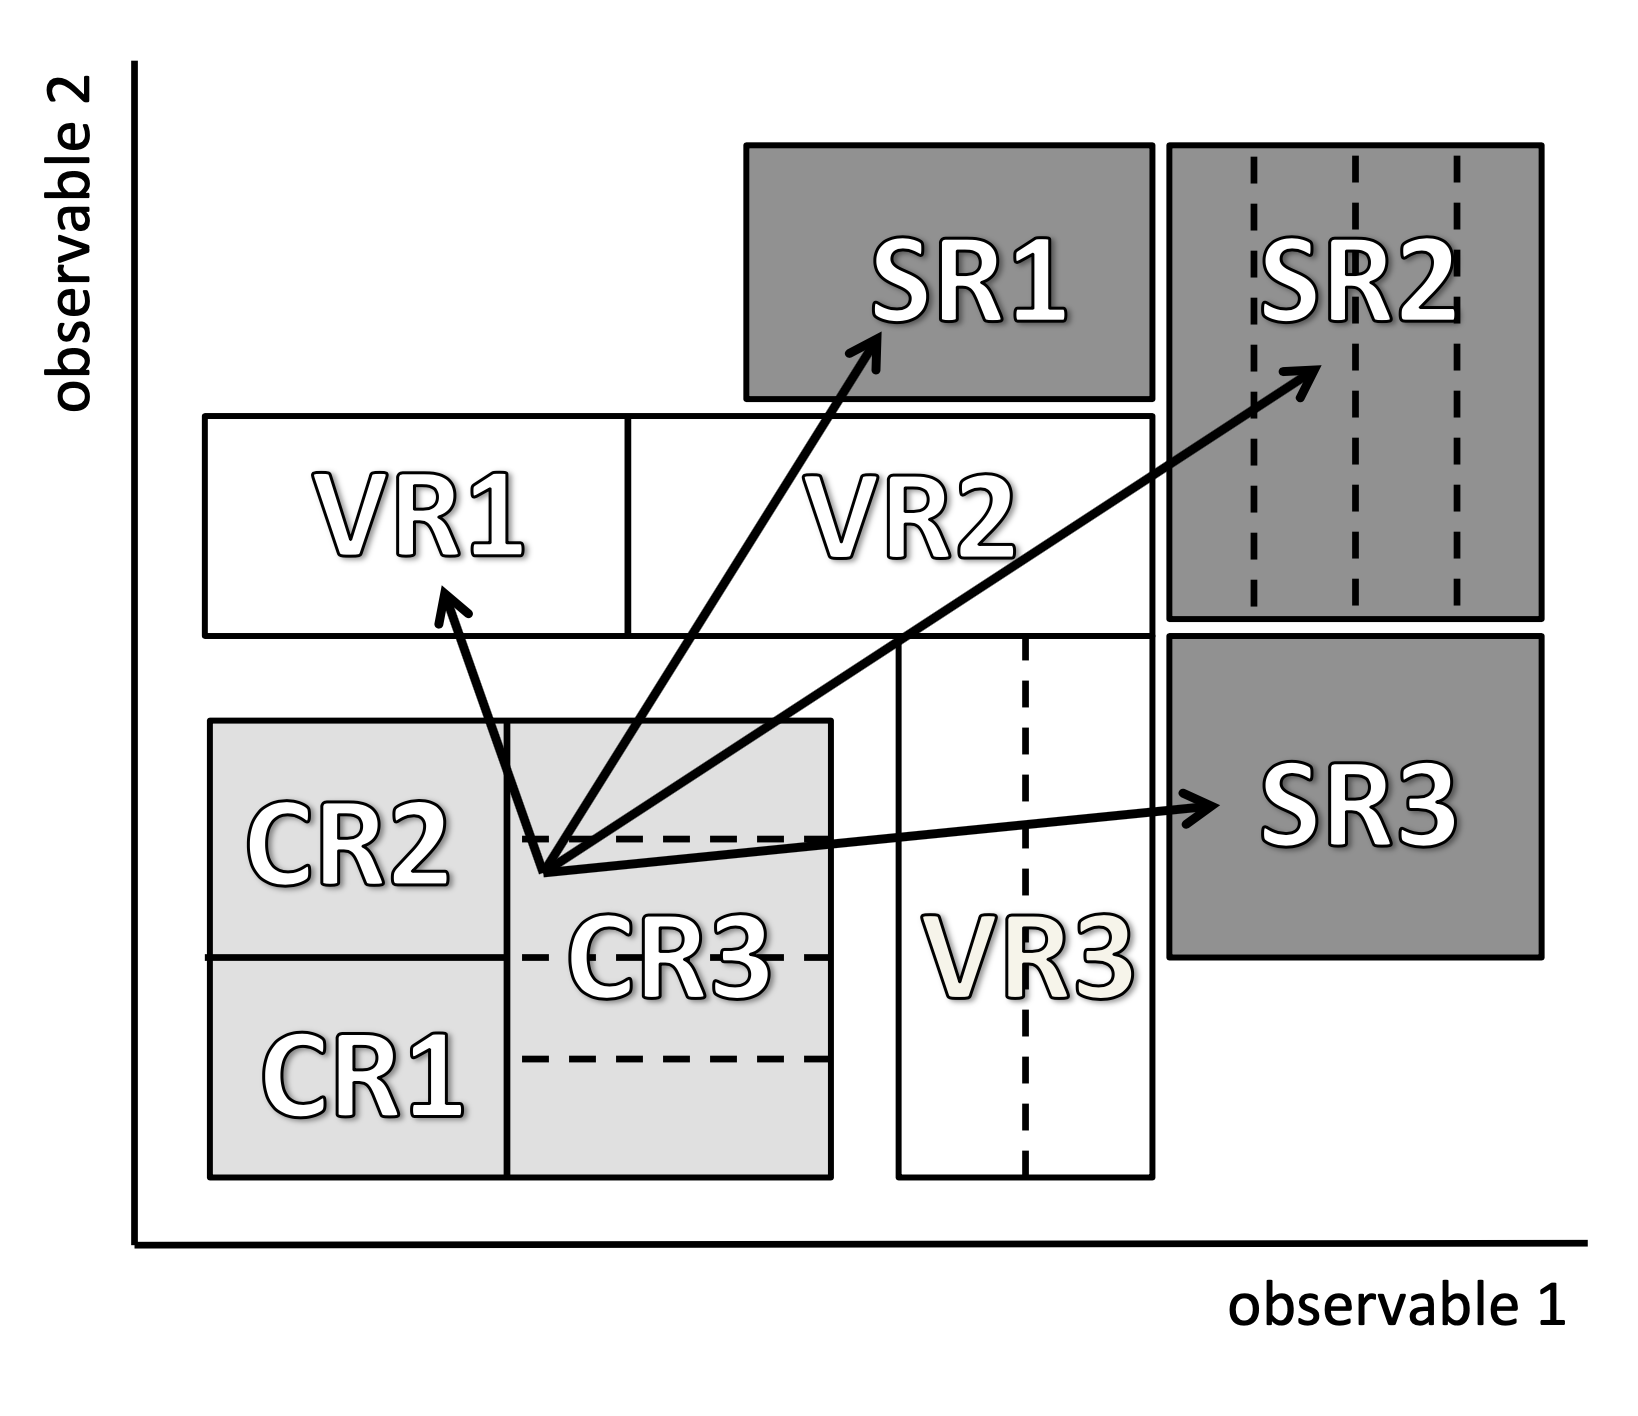
\includegraphics[width=0.45\textwidth]{hf_strategy}}
\end{figure}

\subsection{Analysis blinding}

An important concept in the design phase of searches for new physics is the idea of \textit{blinding} regions of interest~\cite{blind:2003rw}, meaning that measured data are not looked at in these regions. This avoids issues of \textit{experimenter's bias}, \ie unintended influences on the design of the analysis based on the observed data. If data were already known when designing the signal regions (and therefore the outcome of the analysis would be known to some extent), experimenter's bias could for example occur during the selection of the final signal region definitions.

During the design of a search for \gls{susy}, signal regions are generally kept blinded until the complete analysis strategy is fixed. Once the \glspl{sr} have been designed, the next step is to develop a suitable background estimation strategy, often involving the introduction of \glspl{cr} with negligible signal contamination. This is then often followed by the design of \glspl{vr} that can be unblinded once the \glspl{cr} are fixed. The \glspl{sr} are only unblinded after the extrapolation of the background estimate (obtained using a background-only fit) from the \glspl{cr} has been verified in the \glspl{vr}, allowing to either quantify potential excesses in data or set limits on model parameters. 

\subsection{Data versus Monte Carlo plots}

In this chapter, all plots comparing data versus \gls{mc} are so-called \textit{pre-fit} plots, meaning that no background-only fit has been run in order to determine the normalisation factors and total systematic uncertainties for the background estimate. Instead, the contributions from the dominant backgrounds $\ttbar$, $\wjets$ and single top are normalised simultaneously in the control regions by solving the system of $i$ equations
\begin{equation}
%	\begin{split}
		n_\mathrm{data}^{\mathrm{CR}_i} = \mu_{\ttbar} B_{\ttbar}^{\mathrm{CR}_i} + \mu_{W} B_{W}^{\mathrm{CR}_i} + \mu_\mathrm{ST} B_\mathrm{ST}^{\mathrm{CR}_i} + B_\mathrm{other}^{\mathrm{CR}_i},
%	\end{split}
\end{equation}
where $i$ runs over the list of \glspl{cr} introduced in \cref{sec:control_regions} and $\mu_{\ttbar}$, $\mu_\mathrm{W}$ and $\mu_\mathrm{ST}$ are the normalisation factors of the $\ttbar$, $\wjets$ and single top backgrounds, respectively, that are to be determined. $B_{\ttbar}^{\mathrm{CR}_i}$, $B_\mathrm{ST}^{\mathrm{CR}_i}$, $B_\mathrm{ST}^{\mathrm{CR}_i}$ and $B_\mathrm{other}^{\mathrm{CR}_i}$ are the background rates expected from \gls{mc} simulation in the \textit{i}-th \gls{cr}. The normalisation factors obtained are 0.96 for $\ttbar$, 1.24 for $\wjets$ and 0.73 for single top. As will be shown in~\cref{sec:results_background_only}, the normalisation factors obtained using the full statistical procedure will be close to these values.

Additionally, the uncertainty bands on the background estimate will include only \gls{mc} statistical uncertainty as well as experimental uncertainties. The variations of the experimental uncertainties are normalised to the nominal background estimate in the case of $\ttbar$, $\wjets$ and single top, such that only the shapes of the dominant backgrounds are affected. For the remaining minor backgrounds, the experimental uncertainties can affect both normalisation and shape. All experimental uncertainties are assumed to be fully correlated over all processes and bins, allowing them to summed in quadrature. Finally, the uncertainty bars on the data points are obtained by assuming data to be Poisson distributed and correspond to the 68\% confidence interval. 

\section{Control regions}\label{sec:control_regions}

\begin{table}
\begin{center}
\resizebox{\textwidth}{!}{
\begin{tabular} {l | c c c | cccccc}
\toprule
\textbf{CR} & \textbf{TR-LM} &  \textbf{TR-MM} &  \textbf{TR-HM} &  \multicolumn{3}{c}{\textbf{WR}} & \multicolumn{3}{c}{ \textbf{STR}} \\                 
\midrule
$\mbb$ [$\GeV$]  & \multicolumn{3}{c|}{$<$100 or $>$140} & \multicolumn{3}{c}{$\in[50,80]$} &\multicolumn{3}{c}{$>$195}\\
$\mt$ [$\GeV$]   & $\in[100,160]$ & $\in[160,240]$ & $>$240 & \multicolumn{3}{c}{$\in[50,100]$} &\multicolumn{3}{c}{$>$100}\\
$\mct$ [$\GeV$]  &\multicolumn{3}{c|}{$<$180} & \multicolumn{3}{c}{$>$180} &\multicolumn{3}{c}{$>$180}\\
\midrule
\textbf{VR} & \textbf{VR-onLM} &  \textbf{VR-onMM} & \textbf{VR-onHM} & \multicolumn{2}{c}{ \textbf{VR-offLM}} &  \multicolumn{2}{c}{\textbf{VR-offMM}} &  \multicolumn{2}{c}{\textbf{VR-offHM}}\\
\midrule
$\mbb$ [$\GeV$]  & \multicolumn{3}{c|}{$\in[100,140]$} & \multicolumn{2}{c}{$\in[50,80]\, \cup [160, 195]$} & \multicolumn{2}{c}{$\in[50,80]\, \cup [160, 195]$}& \multicolumn{2}{c}{$\in[50,75]\, \cup [165, 195]$}\\
$\mt$ [$\GeV$]   & $\in[100,160]$ & $\in[160,240]$ & $>$240 & \multicolumn{2}{c}{$\in[100,160]$} & \multicolumn{2}{c}{$\in[160,240]$} & \multicolumn{2}{c}{$>$240}\\
$\mct$ [$\GeV$]  &\multicolumn{3}{c|}{$<$180}&\multicolumn{6}{c}{$>$180}\\
\bottomrule
\end{tabular}}
\caption{Overview of the CR and VR definitions. With the exception of $\mlb$, which is not used in the definitions of the \glspl{cr} and \glspl{vr}, all regions share the same selection as the \glspl{sr} on the remaining kinematic observables not listed here.} 
\label{tab:CRVRdef}
\end{center}
\end{table}

The contributions from $\ttbar$, $\wjets$ production and single top processes are normalised to data in dedicated control regions. Other processes like $Z+\mathrm{jets}$, diboson and multiboson, $\ttbar+V$, $\ttbar+h$ and $V+h$ are estimated directly from \gls{mc} simulation and normalised to their theoretical cross sections. All \glspl{cr} are designed to be kinematically as close as possible to the respective \glspl{sr}, such that the normalisation factors derived in the \glspl{cr} are also valid in the \glspl{sr}. The \glspl{cr} are mutually exclusive and made orthogonal to the \glspl{sr} through their requirements on $\mt$, $\mct$ and $\mbb$. Apart from the requirements on these three observables, as well as the requirement on $\mlb$ (removed altogether in the \glspl{cr}), the \glspl{cr} share the same set of cuts as the \glspl{sr}. \Cref{fig:cr_strategy} illustrates the configuration of all \glspl{cr}, especially highlighting the fact that all \glspl{cr} are located in sideband regions off the $\mbb$ window, significantly reducing signal contamination. \Cref{tab:CRVRdef} summarises the kinematic requirements separating the \glspl{cr} from other regions of interest in the analysis. The pre-fit distributions of all \glspl{cr} in representative observables are shown in~\cref{fig:CR_distributions_prefit}.

\subsubsection[Control regions for $\ttbar$]{Control regions for $\boldsymbol{\ttbar}$}

As events from $\ttbar$ processes constitute the dominant \gls{sm} background in all \glspl{sr}, it is necessary to have a precise and reliable estimate of their contributions. Three \glspl{cr} are defined for $\ttbar$, following the same binning in $\mt$, and thus called TR-LM, TR-MM and TR-HM in the following. A good purity of $\ttbar$ processes as well as the necessary high \gls{mc} statistics are achieved  by inverting the requirement on $\mct$, selecting events below the kinematic endpoint for $\ttbar$ processes. The achieved pre-fit $\ttbar$ purities are 79.6\% in TR-LM, 85.9\% in TR-MM and 84.1\% in TR-HM. The remaining contributions stem mostly from single top and $\wjets$ processes and vary between 8.6\%--14.1\% and 1.8\%--4.3\%, respectively, depending on the \gls{sr}. 

For a trustworthy estimate of the contributions from $\ttbar$ processes, it is important that the control regions associated to each signal region exhibit approximately the same composition of $\ttbar$ decay modes. The decay mode most relevant to the \onelepton search at relatively low and moderate values of $\mt$ is the semi-leptonic decay ($\ell\nu qq$), where one of the $W$ bosons decays leptonically, while the other one undergoes a hadronic decay. The semi-leptonic decay mode exhibits the well-known kinematic endpoint in $\mt$ and thus quickly loses importance at high transverse mass values. Events involving a hadronic decay of a $\tau$-lepton originating from $W\to\tau_\mathrm{had}\nu$ in one of the two branches and a leptonic $W$ boson decay in the other branch ($\ell\nu\tau_\mathrm{had}\nu$), are the dominant decay mode in selections with high values of $\mt$. Due to the additional neutrino in such events, the $\ell\nu\tau_\mathrm{had}\nu$ decay mode does not exhibit the same kinematic endpoint as the semi-leptonic one. Finally, di-leptonic decays ($\ell\nu\ell\nu$) and events with a leptonically decaying $\tau$-lepton ($\ell\nu\tau_\mathrm{\ell}\nu$) where one of the two leptons is not reconstructed play a sub-dominant but non-negligible role in all regions. Other $\ttbar$ decay modes are negligible in all analysis selections.

 In the low-mass regions with moderate values in $\mt$ not far above its kinematic endpoint, 80\% (40\%) of $\ttbar$ events involve the semi-leptonic decay mode in the control region (signal region). The sub-dominant decay mode in these regions involves the $\ell\nu\tau_\mathrm{had}\nu$ decay mode, with a contribution of 25\% and 10\% in TR-LM and SR-LM, respectively. Di-leptonic and $\ell\nu\tau_\mathrm{\ell}\nu$ decay modes each contribute about 15\% of all events in TR-LM and about 3\% in SR-LM. Overall, the composition in the low-mass regions is hence not exactly the same in the control and signal regions, but the agreement is still considered to be acceptable.
 With about 45\% (36\%) and 30\% (35\%), the largest contributions in TR-MM (SR-MM) originate from $\ell\nu\tau_\mathrm{had}\nu$ decays and di-leptonic events, respectively. Events with a $\ell\nu\tau_\mathrm{\ell}\nu$ decay contribute to about 10\% (15\%) in TR-MM (SR-MM). 
 In the high-mass control and signal regions with a high requirement on $\mt$, the majority (about 50\%) of events involve the $\ell\nu\tau_\mathrm{had}\nu$ decay mode, while the di-leptonic and $\ell\nu\tau_\mathrm{\ell}\nu$ decay modes contribute with about 30\% and 20\%, respectively. Overall, the compositions of the different $\ttbar$ decay modes in each control region are thus similar to the contributions in the respective signal region, meaning that the proportions of $\ttbar$ processes constrained through the log-likelihood fit in the \glspl{cr} are the same as those to be estimated in the \glspl{sr}.

Signal contamination in the $\ttbar$ \glspl{cr} is avoided by inverting the requirement on $\mbb$, \ie placing the $\ttbar$ \glspl{cr} in the $\mbb$ sideband. The maximum signal contamination over the entire signal grid is 0.8\%, 1.1\% and 1.9\% for TR-LM, TR-MM and TR-HM, respectively, and thus negligible. \Cref{fig:signal_contamination_TRLM,fig:signal_contamination_TRMM,fig:signal_contamination_TRHM} show the signal contamination in the $\ttbar$ \glspl{cr} over the full signal grid. 

 \begin{figure}
	\centering
	\begin{subfigure}[b]{0.5\linewidth}
		\centering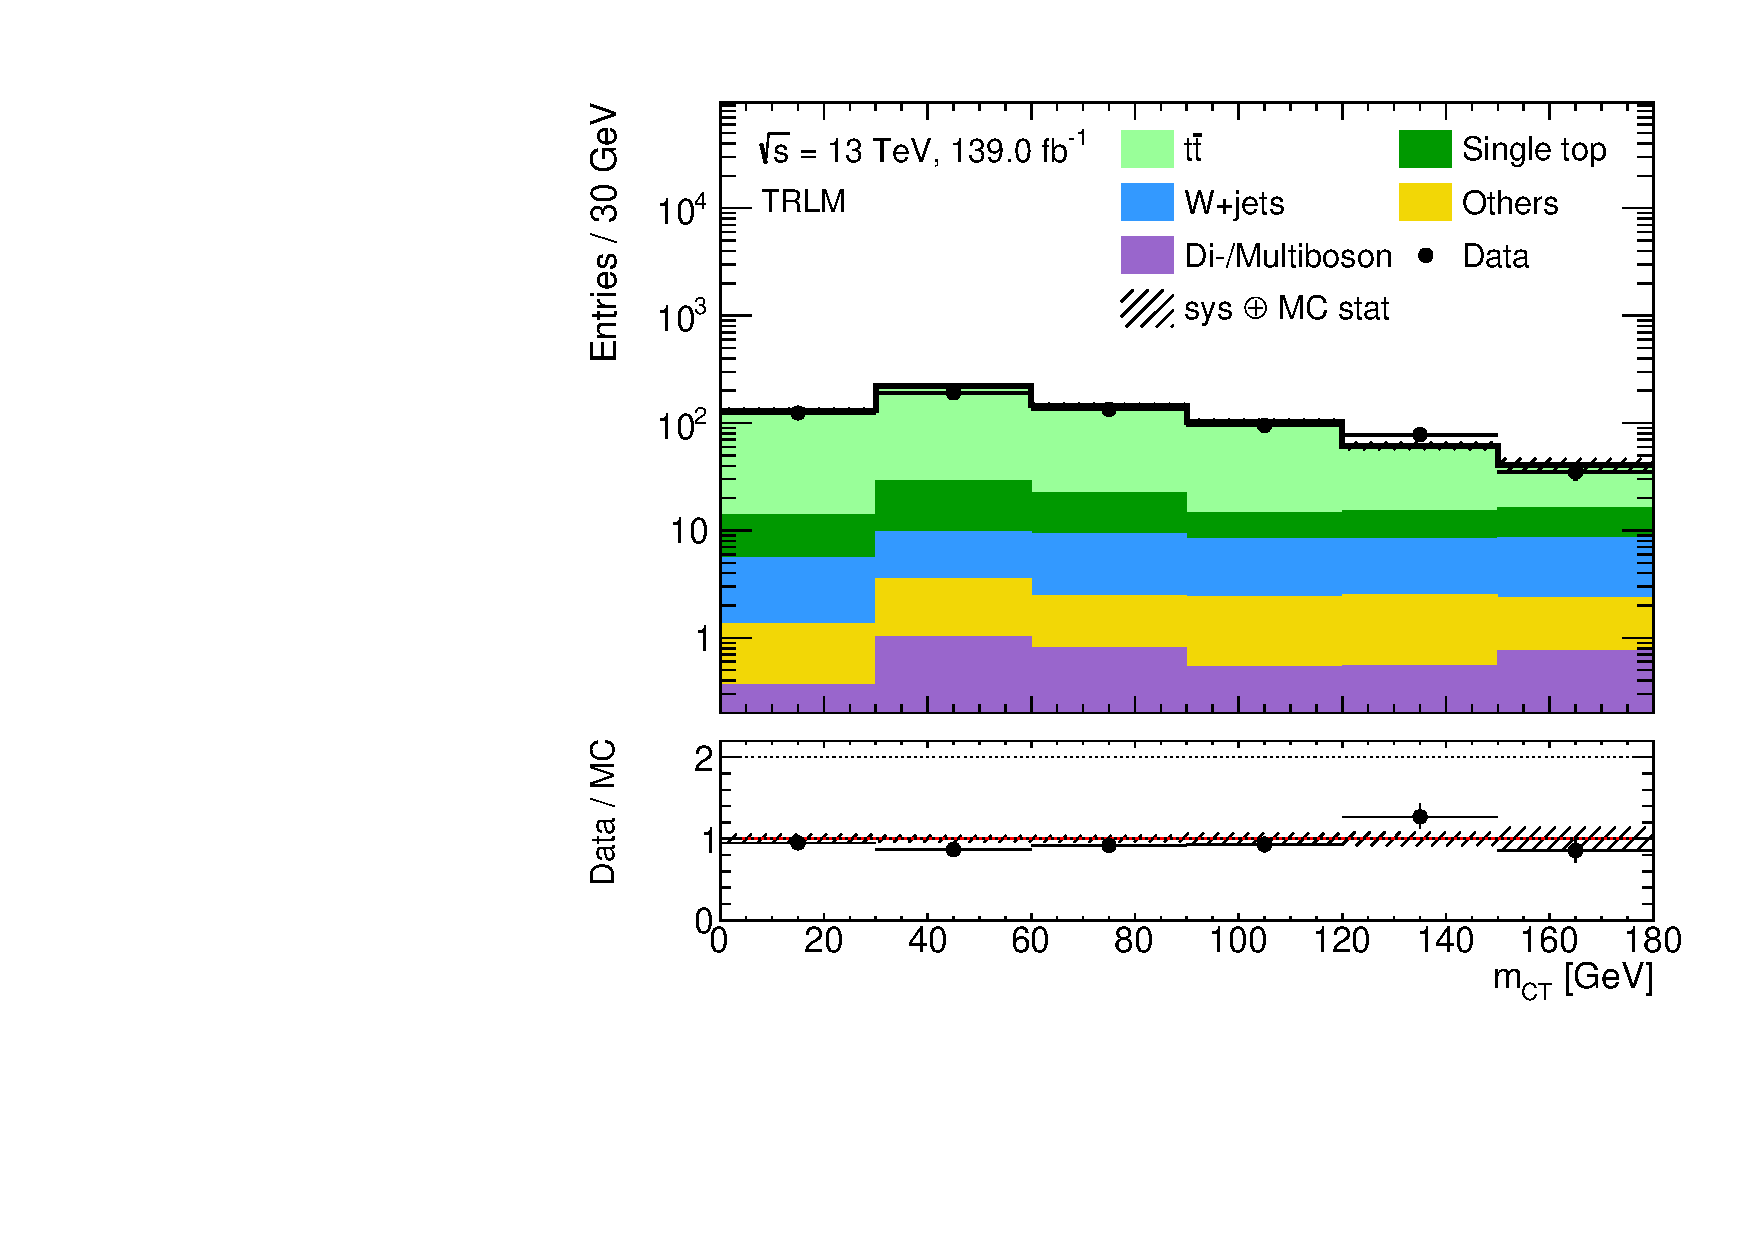
\includegraphics[width=1.0\textwidth]{1Lbb_TRLM_mct}
		\caption{TRLM\label{fig:signal_contamination_TRLM}}
	\end{subfigure}\hfill
	\begin{subfigure}[b]{0.5\linewidth}
		\centering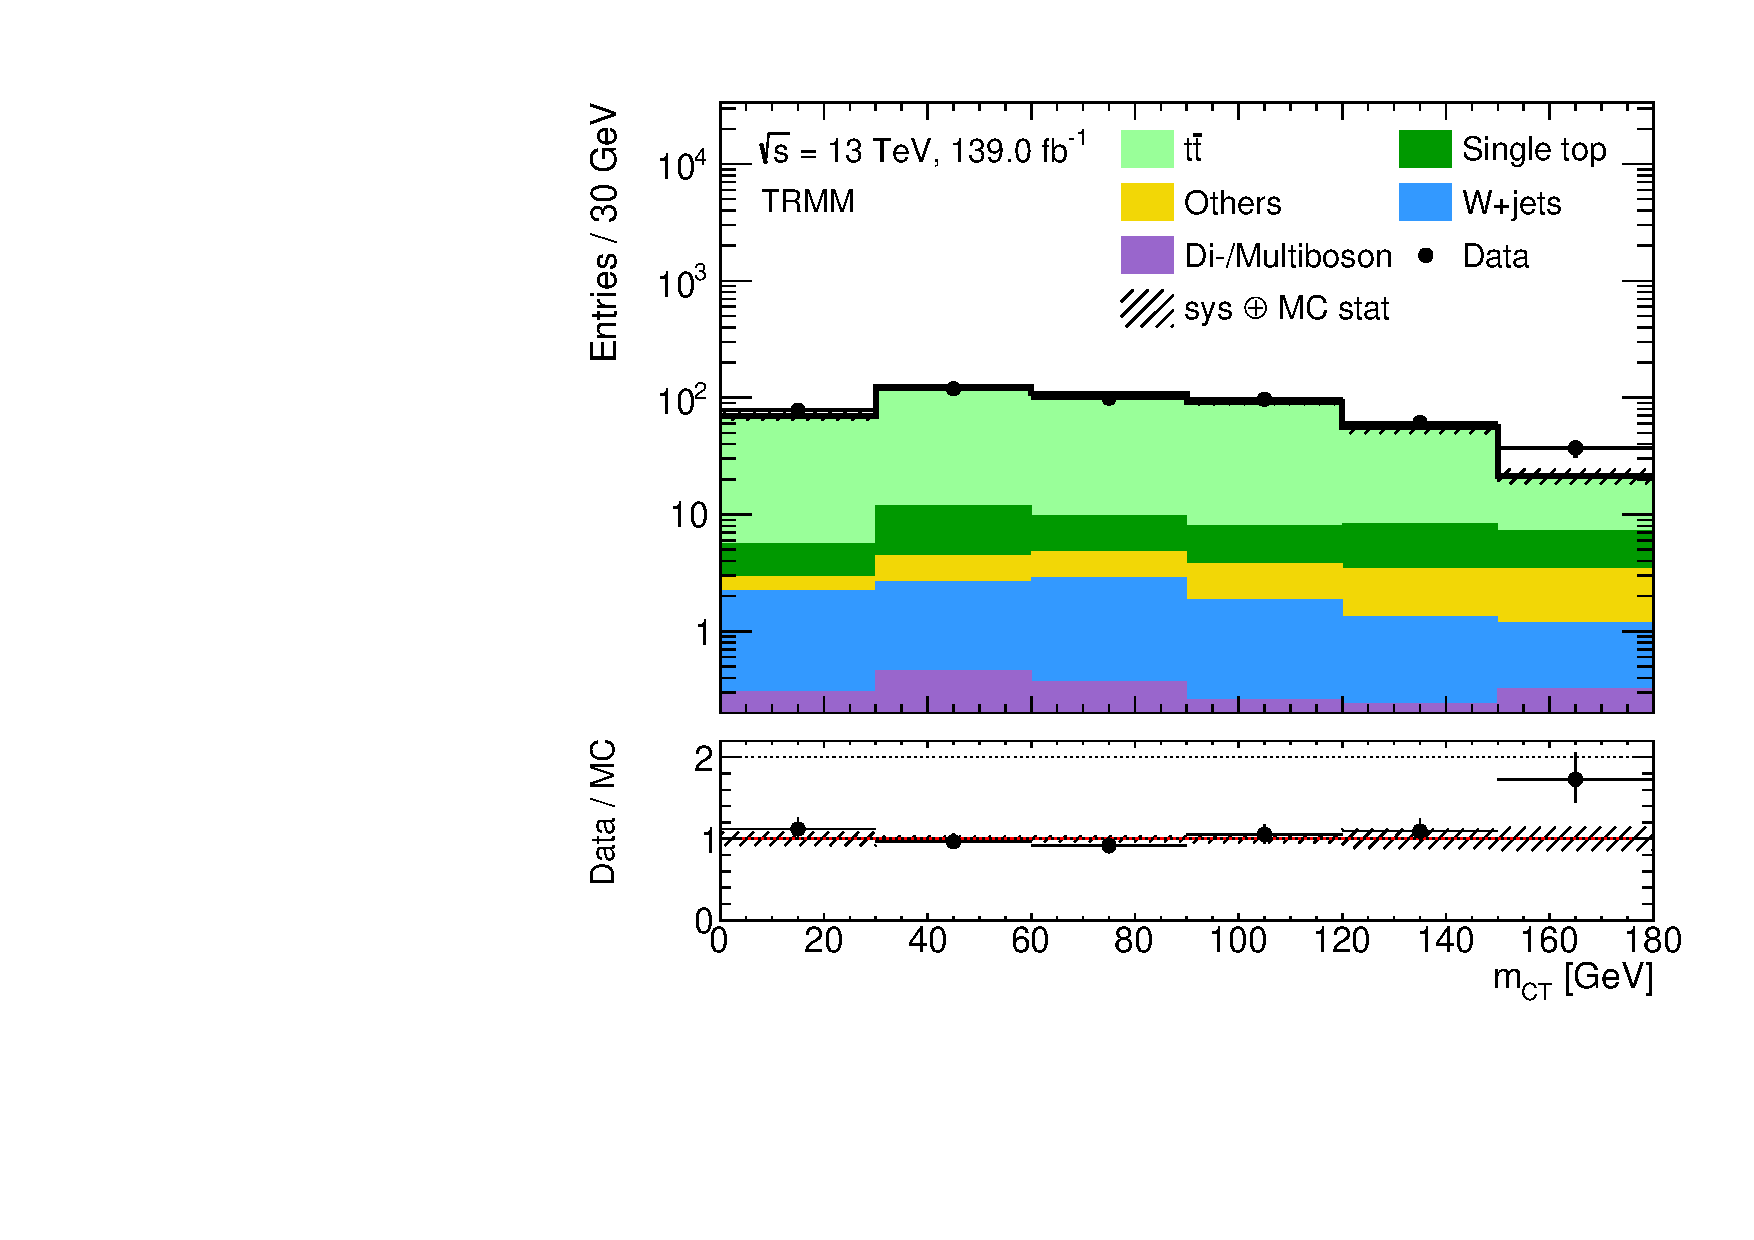
\includegraphics[width=1.0\textwidth]{1Lbb_TRMM_mct}
		\caption{TRMM\label{fig:signal_contamination_TRMM}}
	\end{subfigure}\hfill
	\begin{subfigure}[b]{0.5\linewidth}
		\centering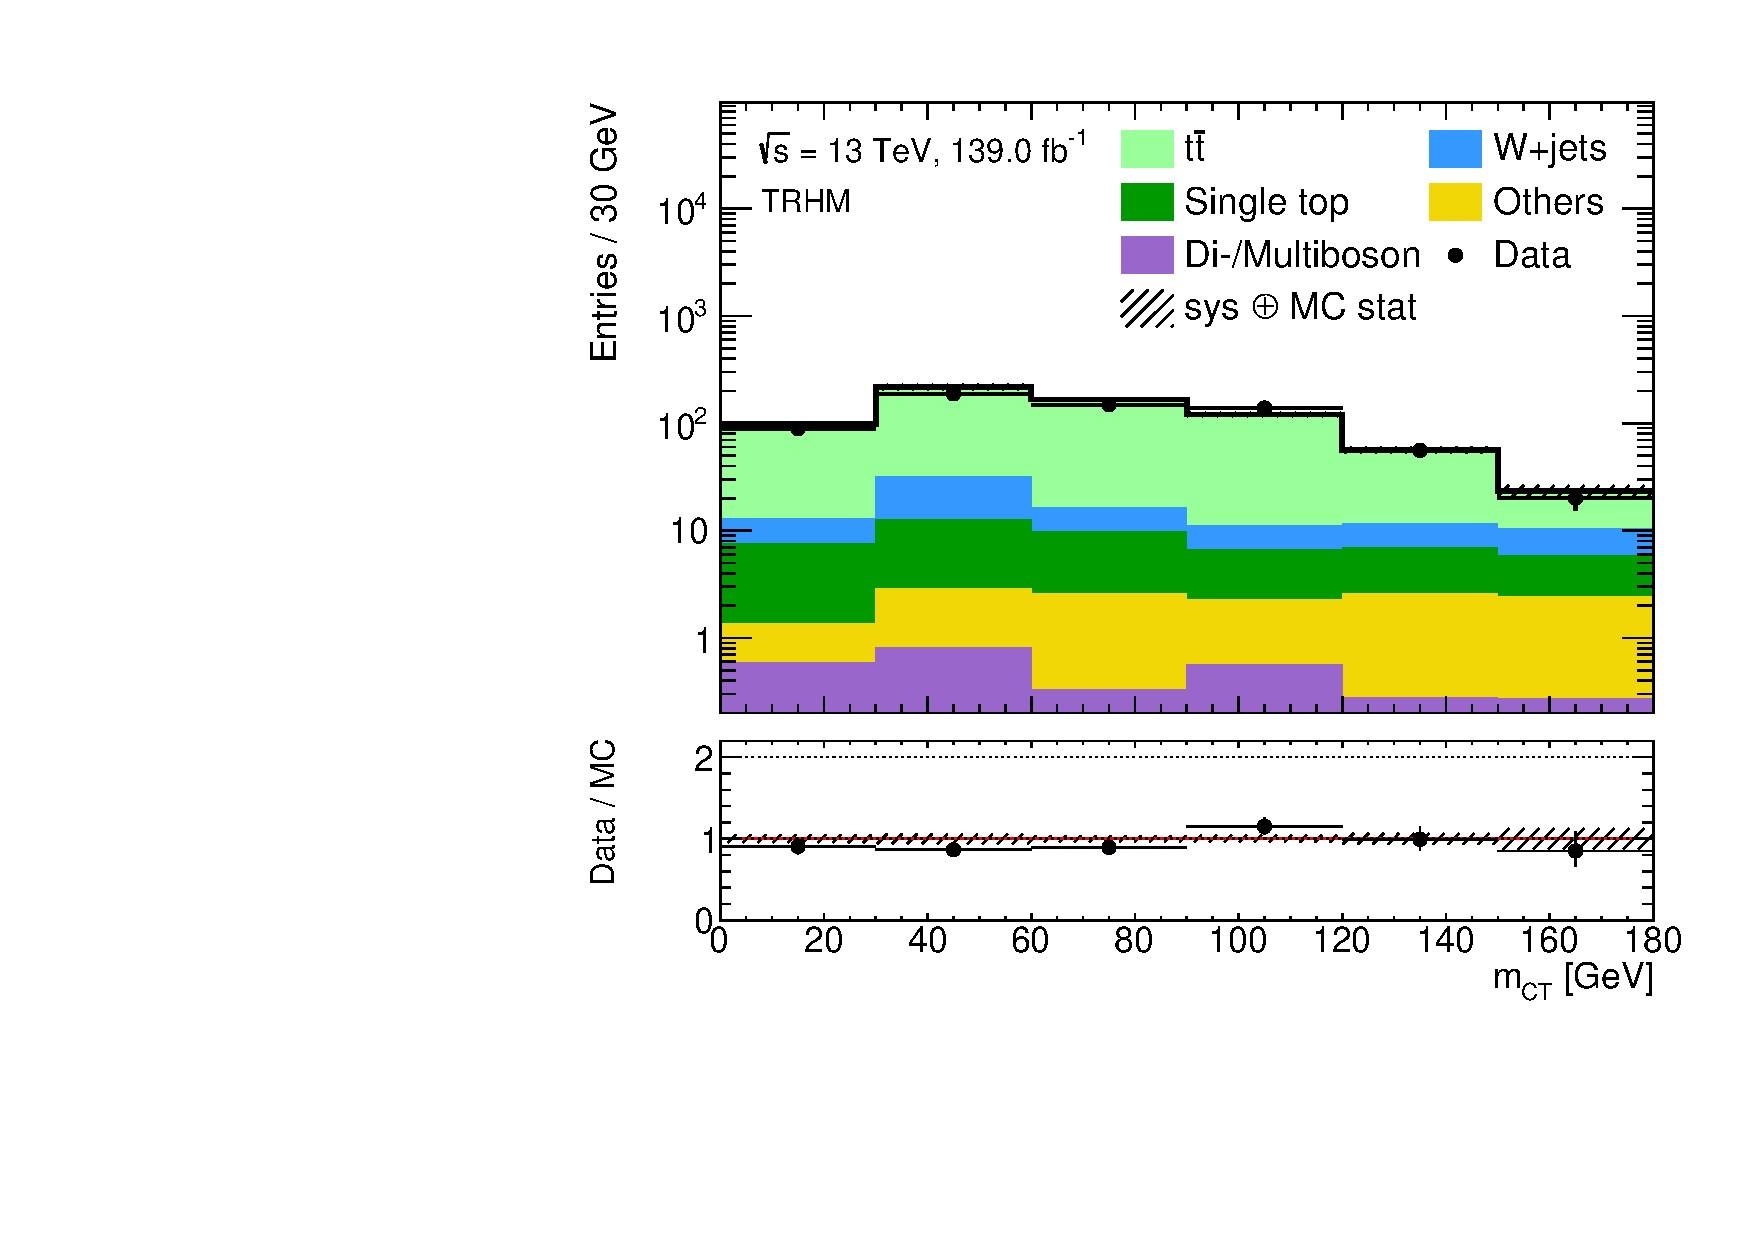
\includegraphics[width=1.0\textwidth]{1Lbb_TRHM_mct}
		\caption{TRHM\label{fig:signal_contamination_TRHM}}
	\end{subfigure}\hfill
	\begin{subfigure}[b]{0.5\linewidth}
		\centering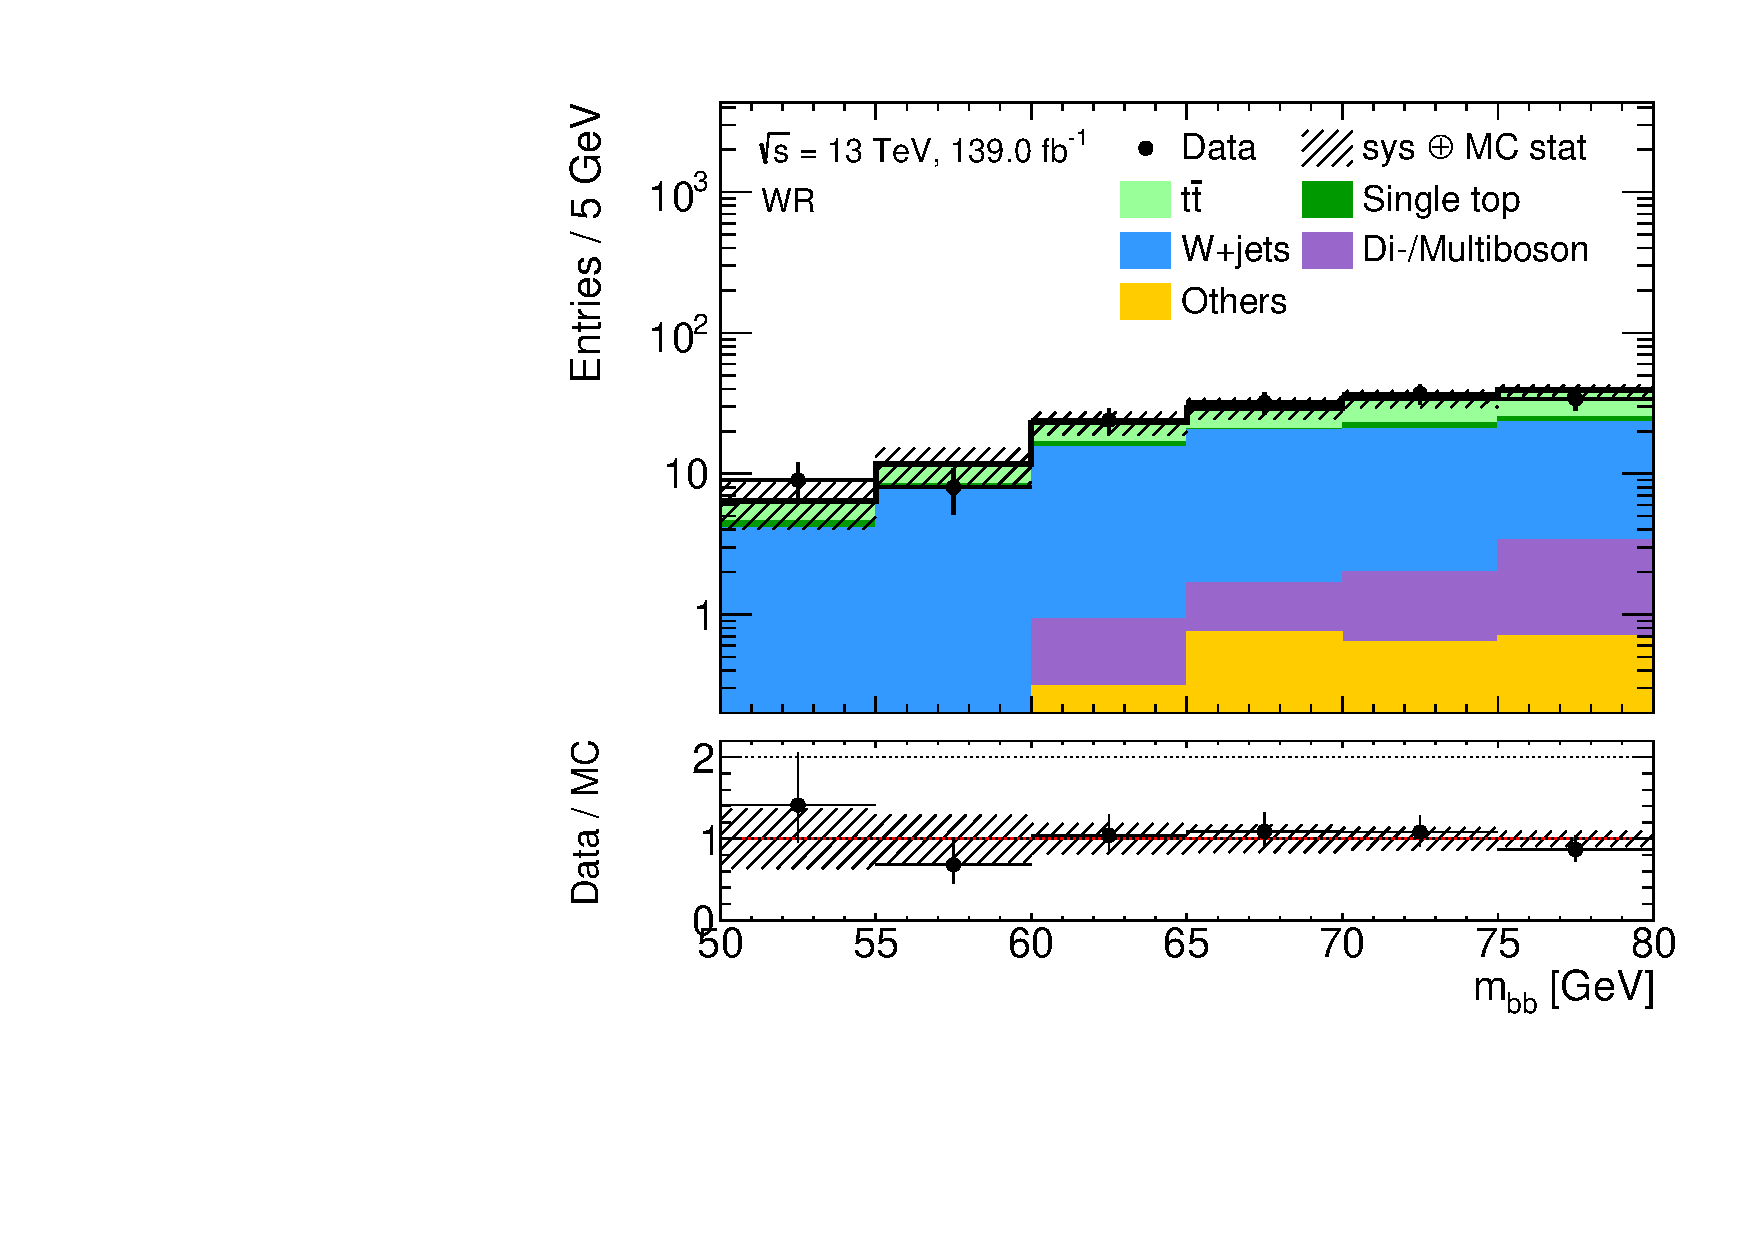
\includegraphics[width=1.0\textwidth]{1Lbb_WR_mbb}
		\caption{WR\label{fig:signal_contamination_WR}}
	\end{subfigure}\hfill
	\begin{subfigure}[b]{0.5\linewidth}
		\centering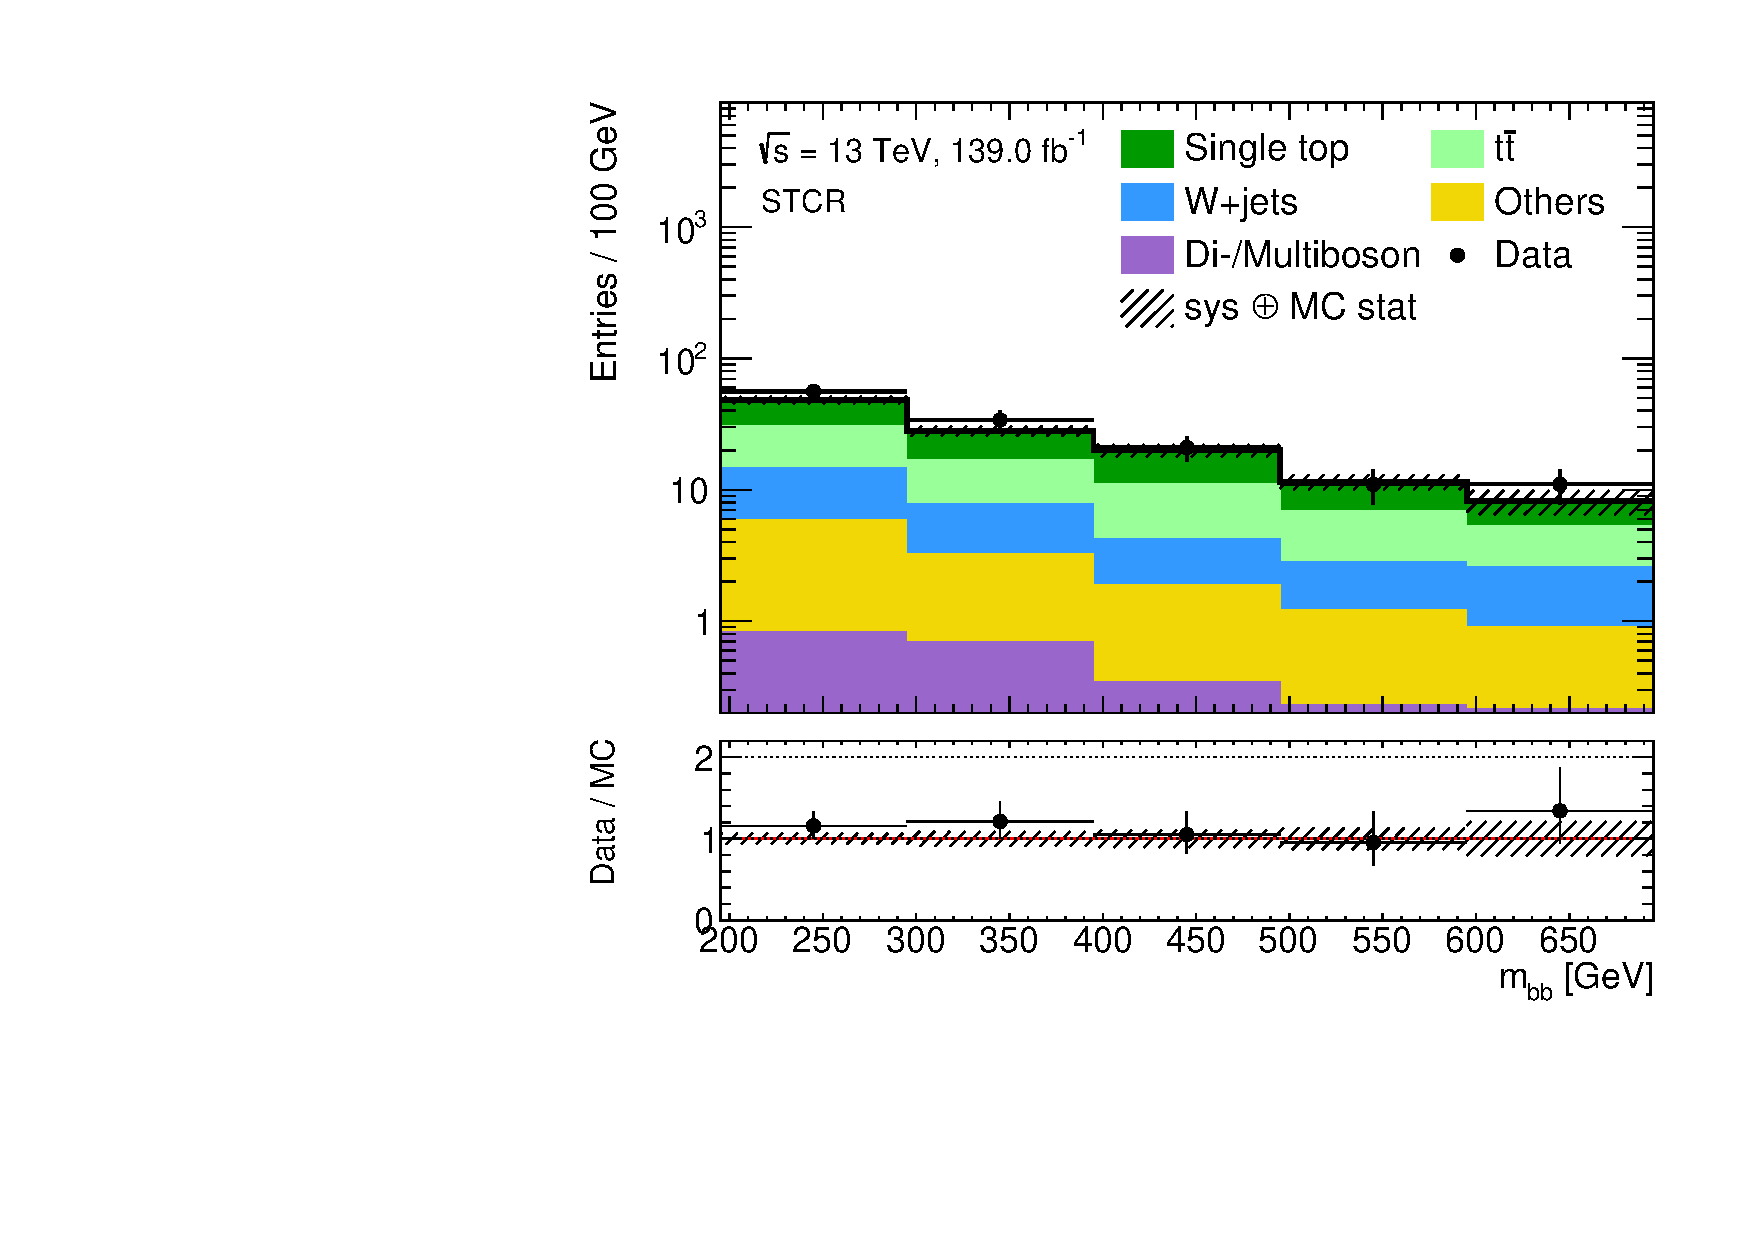
\includegraphics[width=1.0\textwidth]{1Lbb_STCR_mbb}
		\caption{STCR\label{fig:signal_contaminations_STCR}}
	\end{subfigure}\hfill

	\caption{Exemplary pre-fit distributions for each control region. As laid out in the beginning of this chapter, the shaded region includes \gls{mc} statistical uncertainty as well as experimental uncertainties, added in quadrature. A good agreement between \gls{mc} expectation and data is observed in all \glspl{cr}.}
	\label{fig:CR_distributions_prefit}
\end{figure}

 \begin{figure}
	\centering
	\begin{subfigure}[b]{0.5\linewidth}
		\centering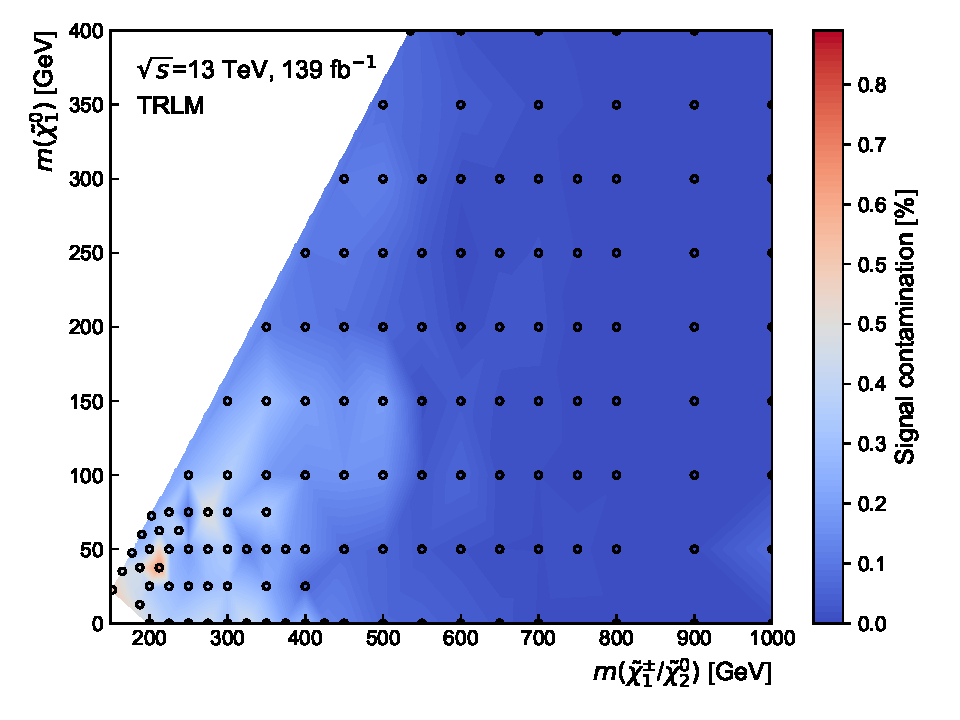
\includegraphics[width=1.0\textwidth]{signal_contamination/plot_TRLM}
		\caption{TRLM\label{fig:signal_contamination_TRLM}}
	\end{subfigure}\hfill
	\begin{subfigure}[b]{0.5\linewidth}
		\centering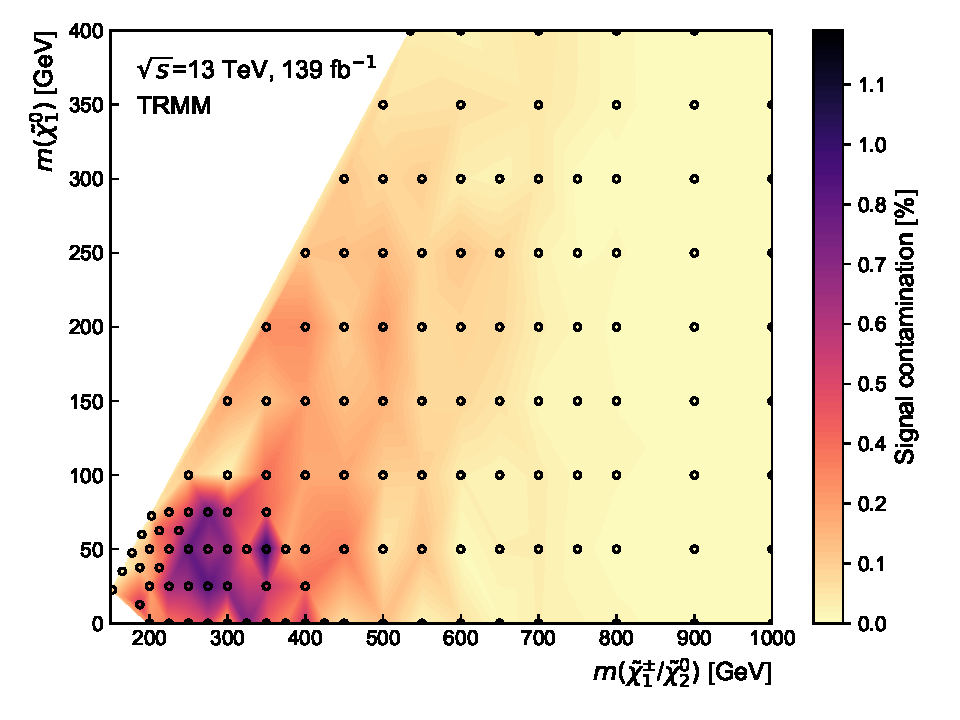
\includegraphics[width=1.0\textwidth]{signal_contamination/plot_TRMM}
		\caption{TRMM\label{fig:signal_contamination_TRMM}}
	\end{subfigure}\hfill
	\begin{subfigure}[b]{0.5\linewidth}
		\centering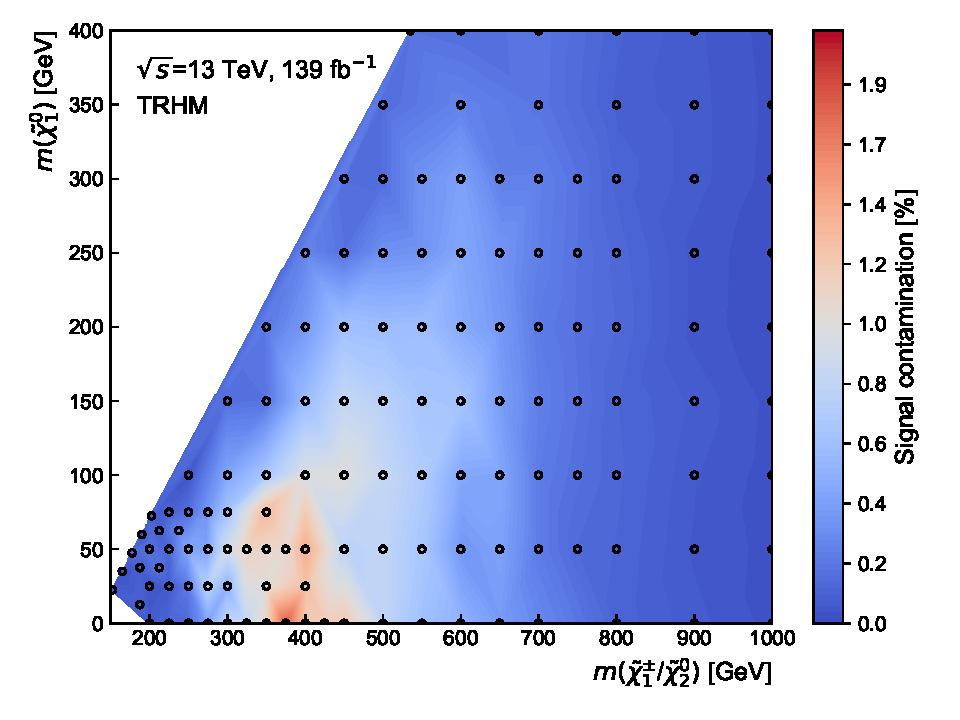
\includegraphics[width=1.0\textwidth]{signal_contamination/plot_TRHM}
		\caption{TRHM\label{fig:signal_contamination_TRHM}}
	\end{subfigure}\hfill
	\begin{subfigure}[b]{0.5\linewidth}
		\centering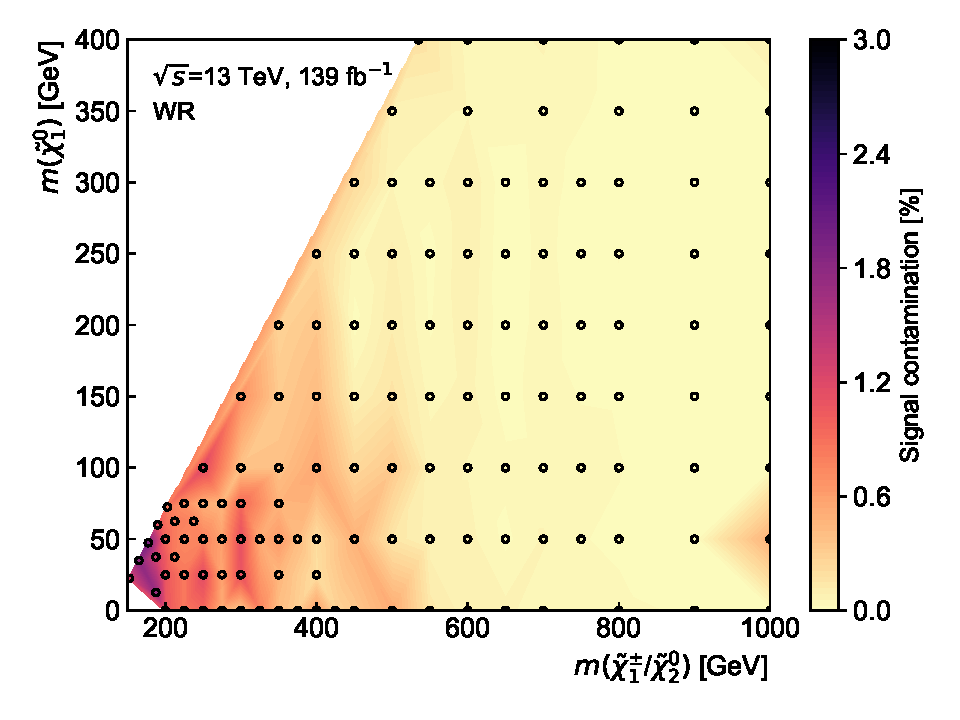
\includegraphics[width=1.0\textwidth]{signal_contamination/plot_WR}
		\caption{WR\label{fig:signal_contamination_WR}}
	\end{subfigure}\hfill
	\begin{subfigure}[b]{0.5\linewidth}
		\centering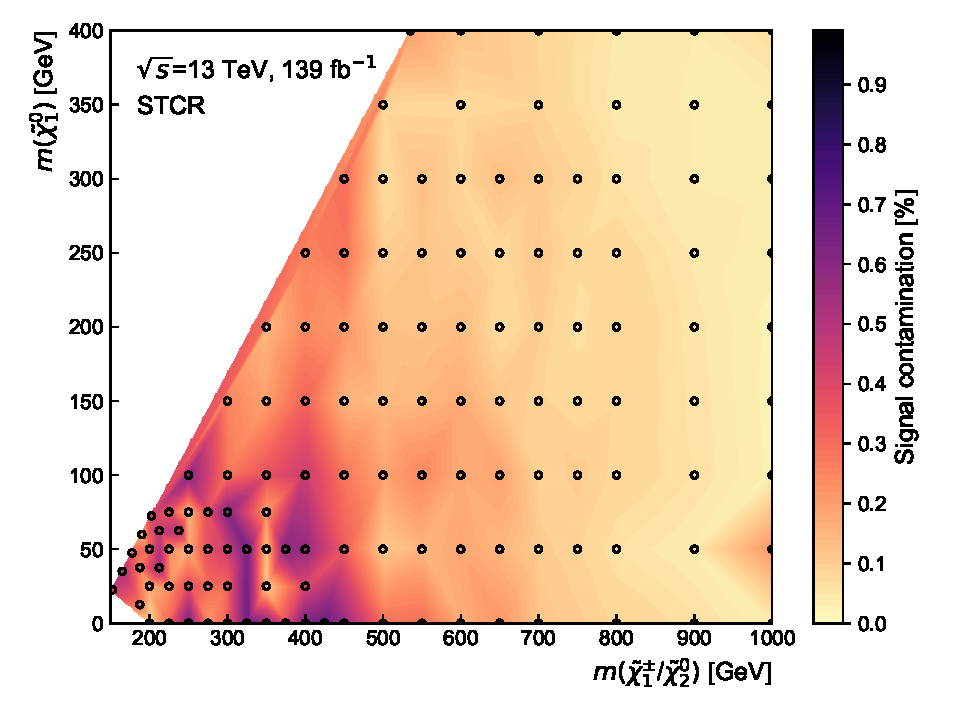
\includegraphics[width=1.0\textwidth]{signal_contamination/plot_STCR}
		\caption{STCR\label{fig:signal_contaminations_STCR}}
	\end{subfigure}\hfill

	\caption{Signal contamination (shown on the \textit{z-axis}) for all \glspl{cr} throughout the signal grid. The space between the signal points (indicated by the black circles) is interpolated using Delaunay triangles.}
	\label{fig:signal_contamination_CR}
\end{figure}

\subsubsection[Control region for $\wjets$]{Control region for $\boldsymbol{\wjets}$}

Events from $\wjets$ production represent the second largest contribution of \gls{sm} background processes in most \glspl{sr}. A single $\wjets$ control region, called WR in the following, is defined by replacing the signal region requirements on $\mt$ and $\mbb$ with $\SI{50}{\GeV} < \mt < \SI{100}{\GeV}$  and $\SI{50}{\GeV} < \mbb < \SI{80}{\GeV}$, respectively. No bins in $\mct$ or $\mt$ are defined for WR, as the composition of $\wjets$ is approximately constant in all regions.

Applying a low requirement on $\mt$ allows to predominantly select events below the kinematic endpoint of the transverse mass of the W boson, resulting in a high statistics control region with a pre-fit $\wjets$ purity of roughly 52.5\%. The sub-dominant background component of WR is $\ttbar$ with 35.2\%. Minor contributions of 7.0\% and 4.2\% originate from single top and diboson processes, respectively. The composition of $\wjets$ events in WR and all signal regions is found to be dominated by $W$ boson production in association with two real \textit{b}-jets. Minor contributions originate from processes with mis-tagged \textit{c}-jets or light-flavour jets.

As was the case for the $\ttbar$ control regions, placing WR off the Higgs mass peak allows to achieve a tolerable maximum signal contamination of only 2.4\% without affecting the composition of processes in the $\wjets$ background too much. Most signal points have significantly less than 1\% signal contamination in WR, as can be seen in~\cref{fig:signal_contamination_WR}. 


\subsubsection{Control region for single top}

Single top processes result in significant background contributions in some \glspl{sr}, necessitating a proper semi-data-driven estimation. A single top \gls{cr} (STR) is defined starting from the \glspl{sr} by replacing the Higgs mass window cut on $\mbb$ with $\mbb > \SI{195}{\GeV}$ and removing the bins in $\mct$. 

The sideband approach achieves again a low maximum signal contamination of roughly 0.8\%. The signal contamination across the entire signal grid is shown in \cref{fig:signal_contaminations_STCR}. The pre-fit purity of the single top processes in STR is 51.7\% and sub-dominant contributions arise from $\ttbar$ processes (29\%), $\wjets$ (10\%) and $\ttbar+V$ (6\%) production. 

 \begin{figure}[t]
	\centering
	\begin{subfigure}[b]{0.5\linewidth}
		\centering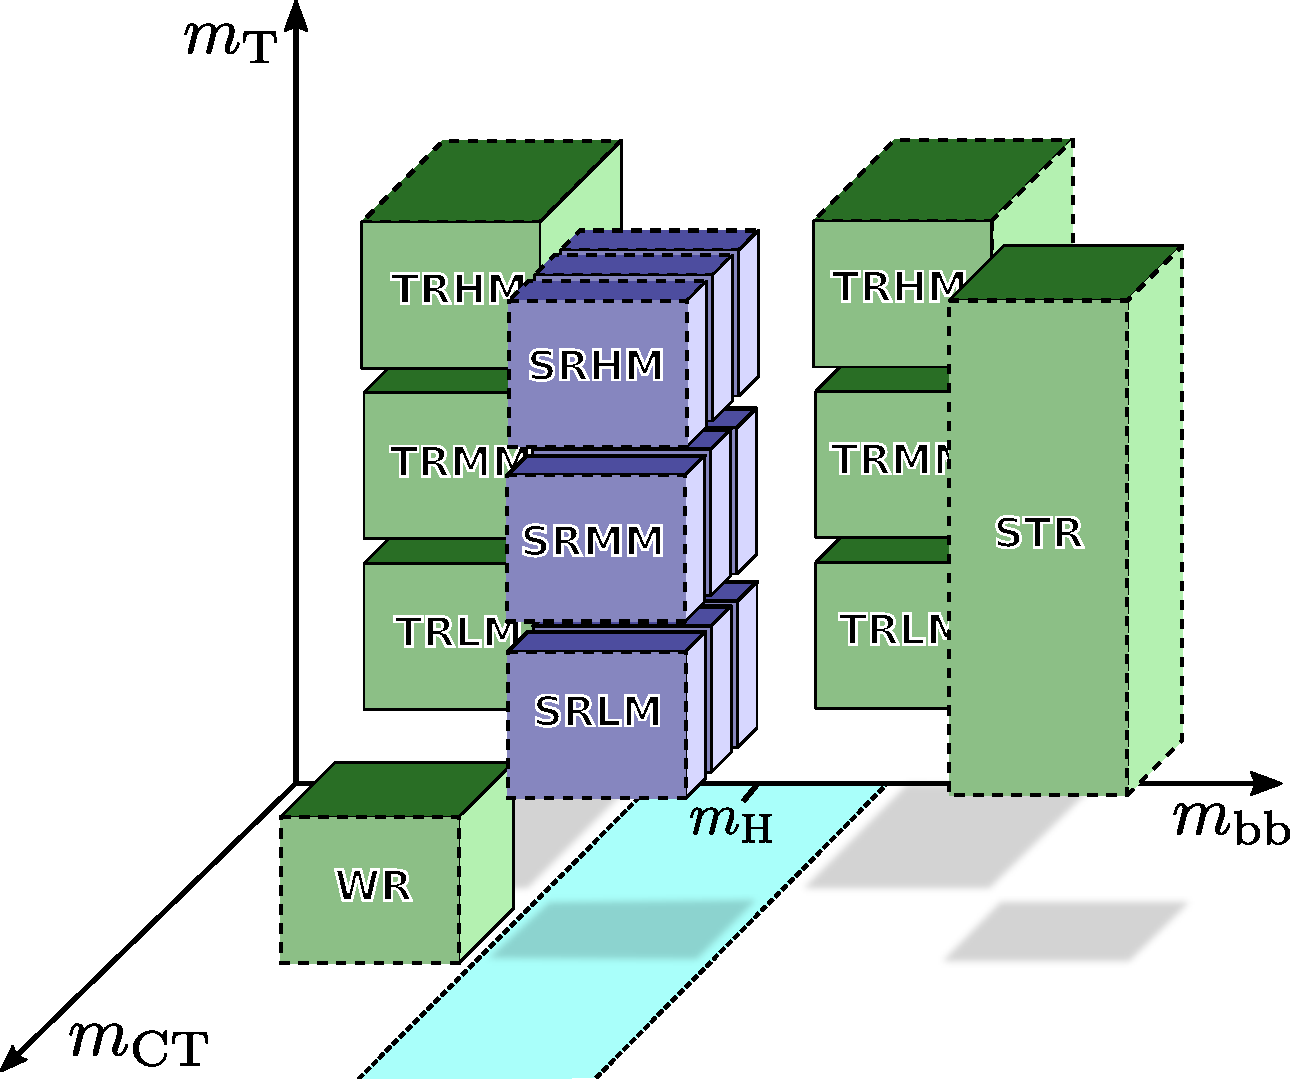
\includegraphics[width=1.0\textwidth]{strategy_5}
		\caption{\label{fig:cr_strategy}}
	\end{subfigure}\hfill
	\begin{subfigure}[b]{0.5\linewidth}
		\centering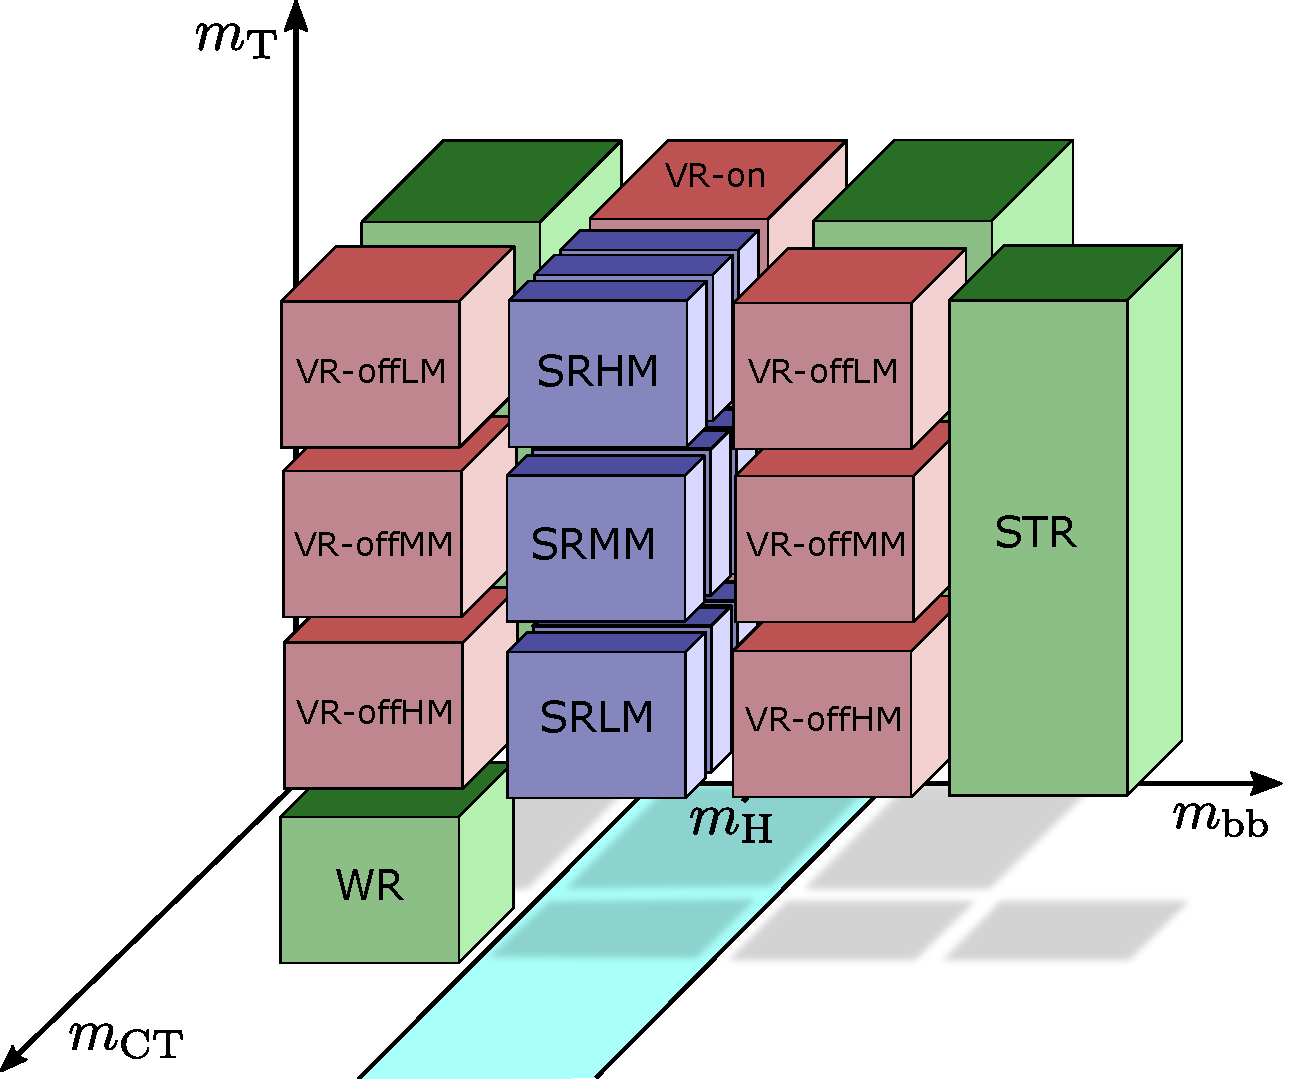
\includegraphics[width=1.0\textwidth]{strategy_7}
		\caption{\label{fig:vr_strategy}}
	\end{subfigure}\hfill

	\caption{Configuration of \subref{fig:cr_strategy} the \glspl{cr} placed around the \glspl{sr} off the $\mbb$ window as well as \subref{fig:vr_strategy} the validation regions in the phase space between the \glspl{cr} and \glspl{sr}. The \glspl{vr} are arranged such that each of the extrapolations can be validated separately for SR-LM, SR-MM and SR-HM.}
	\label{fig:results_HF_scans}
\end{figure}

\section{Validation regions}


Two sets of \glspl{vr} regions are introduced in order to verify the extrapolations over the different distributions. The selections defining all \glspl{vr} are summarised in \cref{tab:CRVRdef}. The first set, called VR-on is situated on the Higgs boson mass peak but with the $\mct$ requirement inverted to $\mct<\SI{180}{\GeV}$. This allows the VR-on regions to validate the extrapolation over $\mct$, performed when extrapolating the background estimate from the $\ttbar$ control regions into the signal regions. Three disjunct VR-on regions are introduced, with $\mt$ requirements matching those of the \glspl{sr}, such that the extrapolations can be validated separately for each signal region. The three VR-on regions are aptly named VR-onLM, VR-onMM and VR-onHM. A similar composition of $\ttbar$ decay modes as in the control and signal regions is observed in the VR-on regions, necessary for a trustworthy validation of the $\ttbar$ estimate. A maximum signal contamination of about 5\%--14\% is achieved, depending on the requirement in $\mt$. As can be seen from~\cref{fig:signal_contaminations_VRs}, most signal points have a signal contamination well below 5\% for all VR-on regions.  

 The second set of \glspl{vr} is located on both sides off the Higgs boson mass peak at same values in $\mct$ than the \glspl{sr}. This set of \textit{off-peak} \glspl{vr}, called VR-off, is used to validate the extrapolation in $\mbb$ and $\mt$. Similar to the on-peak validation regions, the VR-off regions are split into bins in $\mt$ matching the signal regions. The resulting validation regions VR-offLM, VR-offMM and VR-offHM, can thus be used to validate the background estimate in their respective signal region. The maximum signal contamination in the VR-off regions is found to be about 7\%--13\%, depending on the requirement on $\mt$. Most signal points, however, reveal a signal contamination in the VR-off regions of less than 3\% (cf.~\cref{fig:signal_contaminations_VRs}).


